\documentclass[11pt]{article}
\usepackage[margin=0.3in,top=0.25in,bottom=0.4in]{geometry}
\makeatletter
\renewcommand{\@maketitle}{\newpage\null\vskip -3.5em\begin{center}{\LARGE \@title \par}\end{center}\par\vskip 0.2em}
\makeatother
\usepackage{amsmath,amssymb}
\usepackage{graphicx}
\usepackage{booktabs}
\usepackage{hyperref}

\title{Our Pb--Pb photon flux compared with Guzey, Innocenti, Sta\'sto and Strikman\\
(arXiv:2606.05469)}
\author{}
\date{}

\begin{document}
\maketitle

\section{Summary}

Guzey \textit{et al.}\ (arXiv:2606.05469, ``GISS'' below) and our default \texttt{FLUX\_MODEL=EFF}
use the same ingredients: the Woods--Saxon photon flux of a point source, the Glauber
survival factor $\Gamma_{AA}$ with $\sigma_{NN}=92$~mb, and the no-EMD probability
$P_{\text{no-EM}}(b)=\exp(-S/b^2)$ with $S=(17.4\,\text{fm})^2$. They differ in
\emph{where} the flux is evaluated:
\begin{itemize}
\item GISS, Eq.~(20): at the \emph{centre} of the target nucleus, a distance $b$ from the
  centre of the photon emitter.
\item EFF (Eskola, Guzey, Helenius, Paakkinen, Paukkunen, arXiv:2404.09731, Eq.~(4)): at the
  position of the struck \emph{nucleon}, averaged over the nucleons of the target with weight
  $T_A$. GISS cite this refinement (their Ref.~[16]) below their Eq.~(15) and say that it
  ``somewhat increases $f_{\gamma/A}(z)$ for large $z$'', but do not use it.
\end{itemize}
The two agree to 1--3\% for $z\lesssim 10^{-3}$. EFF is larger by 11\% at $z=10^{-2}$, by a
factor of 1.7 at $z=0.03$ and by a factor of 30 at $z=0.1$. For p--Pb our flux is the same as
GISS. Our \texttt{FLUX\_MODEL=WS} option is exactly the GISS Pb--Pb flux.

\section{The two Pb--Pb fluxes}

Both use $z=\omega/E_A=2\omega/\sqrt{s_{NN}}$ and the flux of a Woods--Saxon charge
distribution at transverse distance $r$ from its centre,
\begin{equation}
  f_{\gamma/A}(z,r)=\frac{\alpha_{\text{em}}Z^2}{\pi^2 z}
  \left|\int_0^\infty dk_\perp\,\frac{k_\perp^2 F_A(k_\perp^2+z^2m_N^2)}{k_\perp^2+z^2m_N^2}\,
  J_1(k_\perp r)\right|^2
\end{equation}
(GISS Eq.~(16); \texttt{flux\_density\_WS} in \texttt{src/photon\_flux.cpp}). The channel factor
is $P_{\text{ch}}(b)=1$ (AnAn), $P_{\text{no-EM}}(b)$ (An0n) or
$P_{\text{no-EM}}(b)\,[1-P_{\text{no-EM}}(b)]$ (Xn0n).

\paragraph{GISS (Eqs.~(15), (20), (22)).}
\begin{equation}
  f^{\text{GISS}}_{\gamma/A}(z)=\int d^2b\; f_{\gamma/A}(z,b)\,\Gamma_{AA}(b)\,P_{\text{ch}}(b).
\end{equation}
The flux is taken at $r=b$, the distance between the two centres.

\paragraph{EFF (arXiv:2404.09731, Eq.~(4); \texttt{init\_effective\_flux}).}
\begin{equation}
  f^{\text{EFF}}_{\gamma/A}(z)=\frac{1}{B}\int d^2r\; f_{\gamma/A}(z,r)\,H(r),\qquad
  H(r)=\int d^2s\; T_A(s)\,\Gamma_{AA}(|\mathbf r-\mathbf s|)\,P_{\text{ch}}(|\mathbf r-\mathbf s|),
\end{equation}
with $\int d^2s\,T_A(s)=B=208$. Here $\mathbf r$ is the position of the struck nucleon measured
from the emitter and $\mathbf s$ its position inside the target, so $b=|\mathbf r-\mathbf s|$.
For $r\gg R_A$, $H(r)\to B\,\Gamma_{AA}(r)P_{\text{ch}}(r)$ and the two fluxes coincide.

\paragraph{Where the interaction point is.} The struck nucleon sits at $\mathbf r=\mathbf b+\mathbf s$,
where $\mathbf s$ is its position measured from the target centre. The weight $T_A(\mathbf s)/B$
is the probability of finding a nucleon there: $(1/B)\int d^2s\,T_A(\mathbf s)=1$, and
$T_A=0$ where there are no nucleons. So the interaction point is distributed over the target
exactly like its nucleons. ``Inside'' means inside a Woods--Saxon nucleus ($R_A=6.49$~fm,
$a=0.54$~fm), not a hard sphere: the code integrates $s$ up to $s_{\max}=R_A+12a\approx13$~fm
(\texttt{init\_effective\_flux}), but beyond $R_A+3a\approx 8$~fm the weight is negligible.

Two things are \emph{not} imposed on the interaction point:
\begin{itemize}
\item No condition relative to the emitter. Only the distance between the two centres,
  $b=|\mathbf r-\mathbf s|$, enters $\Gamma_{AA}$ and $P_{\text{ch}}$, so the hadronic cut acts
  on $b$, not on $r$. The interaction point can be closer to the emitter than the target centre,
  which is what increases the flux. With $b\gtrsim14$~fm and $s\lesssim 8$~fm it never enters the
  emitter's charge distribution ($r\gtrsim 6$--7~fm), so the point-source form of
  $f_{\gamma/A}(z,r)$ remains valid.
\item No cut on $r$ itself. The $\mathbf r$ integral covers the whole plane; configurations with
  small $r$ get zero weight because $\Gamma_{AA}(b)$ vanishes there.
\end{itemize}
A compact way to say it in a paper: \emph{the interaction point $P$ is distributed over the
target according to its nuclear thickness function $T_A(\mathbf s)$.}

\section{The effective flux as implemented in our code}

Everything below is in \texttt{src/photon\_flux.cpp} and \texttt{src/photon\_flux.hpp}
(function \texttt{init\_effective\_flux}), following Eq.~(4) of arXiv:2404.09731.

\paragraph{1. Effective flux.} The number of photons per unit energy is
\begin{equation}
  \frac{dN_\gamma}{d\omega}(z_\gamma)=\frac{1}{B}\int d^2r\;f_{\gamma A}(z_\gamma,\mathbf r)\,H(\mathbf r)
  =\frac{2\pi}{B}\int_0^{r_{\max}} r\,dr\;f_{\gamma A}(z_\gamma,r)\,H(r),
\end{equation}
with $z_\gamma=2\omega/\sqrt{s_{NN}}$, $\omega=q^+/\sqrt2$ the photon energy, $B=208$ the mass number
of the target and $r_{\max}=60/(z_\gamma m_N)$, beyond which the flux is negligible. It is computed
once on 100 points in $\ln z_\gamma\in[\ln10^{-6},0]$ and interpolated with a cubic spline by
\texttt{effective\_photon\_flux(qp)}. With this flux the cross sections have no impact-parameter
integral left.

\paragraph{2. Averaging over the target} (\texttt{EffFluxRadial::H\_raw}):
\begin{equation}
  H(r)=\int d^2s\;T_B(\mathbf s)\;\Gamma_{AA}(|\mathbf r-\mathbf s|)\;P_{\text{ch}}(|\mathbf r-\mathbf s|),
  \qquad \int d^2s\,T_B(\mathbf s)=B .
\end{equation}
$\mathbf r$ is the position of the struck nucleon measured from the emitter, $\mathbf s$ its position
inside the target, and $b=|\mathbf r-\mathbf s|$ the distance between the two centres. $H(r)$ is
tabulated on 400 points in $\ln r$ for $r<800$~GeV$^{-1}\approx160$~fm; beyond that the code uses the
limit $H\to B\,\Gamma_{AA}(r)P_{\text{ch}}(r)$.

\paragraph{3. Ingredients.}
\begin{itemize}
\item Photon density at distance $r$ from the emitter (\texttt{flux\_density\_WS}):
  \begin{equation}
    f_{\gamma A}(z_\gamma,r)=\frac{2\alpha Z^2}{\pi^2 z_\gamma\sqrt{s_{NN}}}
    \left|\int_0^{q_{\max}}dk_\perp\,
    \frac{k_\perp^2F_A\!\left(\sqrt{k_\perp^2+z_\gamma^2m_N^2}\right)}{k_\perp^2+z_\gamma^2m_N^2}\,
    J_1(k_\perp r)\right|^2,
  \end{equation}
  with the Woods--Saxon charge form factor $F_A$, $q_{\max}=5$~GeV and $Z=82$. For $r\geq 14.2$~fm
  it is replaced by the point-charge result (\texttt{flux\_density}), which is identical outside
  the nucleus:
  \begin{equation}
    f_{\gamma A}(z_\gamma,r)=\frac{\alpha Z^2}{\pi^2\omega}\,\frac{\eta^2}{r^2}\,K_1^2(\eta),
    \qquad \eta=z_\gamma m_N r .
  \end{equation}
\item Target thickness $T_B(s)$: Woods--Saxon density with $R_A=6.49$~fm and $a=0.54$~fm,
  normalised to $B$ nucleons, integrated up to $s_{\max}=R_A+12a$.
\item Probability of no hadronic interaction: $\Gamma_{AA}(b)=\exp[-\sigma_{NN}T_{AA}(b)]$, optical
  Glauber with $\sigma_{NN}=92$~mb (\texttt{input/WS\_photon\_flux/Gamma\_AA.dat}).
\item Neutron selection, with $P_{\text{no-EM}}(b)=\exp(-S/b^2)$ and $S=(17.4\,\text{fm})^2$:
  \begin{equation}
    P_{\text{ch}}(b)=
    \begin{cases}
      1 & \text{AnAn},\\
      P_{\text{no-EM}}(b) & \text{An0n},\\
      P_{\text{no-EM}}(b)\,[1-P_{\text{no-EM}}(b)] & \text{Xn0n},\\
      P_{\text{no-EM}}(b)^2 & \text{0n0n}.
    \end{cases}
  \end{equation}
\end{itemize}

\paragraph{Woods--Saxon form factor.} $F_A$ is the Fourier transform of the two-parameter
Woods--Saxon charge density, normalised to $F_A(0)=1$, as in Eqs.~(11)--(13) of arXiv:2404.09731:
\begin{equation}
  F_A(q)=\frac{1}{A}\int d^3x\;\rho_A(|\vec x|)\,e^{i\vec q\cdot\vec x}
  =\frac{4\pi}{A}\int_0^\infty dx\,\frac{x}{q}\,\sin(qx)\,\rho_A(x),\qquad
  \rho_A(x)=\frac{\rho_0}{1+\exp[(x-R_A)/a]},
\end{equation}
with $R_A=6.49$~fm and $a=0.54$~fm. Here $x=|\vec x|$ is the 3D distance from the centre of the
nucleus: the density is spherically symmetric, so it depends only on this modulus. It is not the
transverse position $\mathbf r$ of the photon flux, a 2D vector in the transverse plane on whose
length $r=|\mathbf r|$ the flux depends; $x$ is only an integration variable and disappears once
$F_A(q)$ is computed. Two implementation details (\texttt{WSFormFactor} in
\texttt{photon\_flux.hpp}):
\begin{itemize}
\item It is evaluated in closed form, not by numerical integration. The Fourier transform of a
  Woods--Saxon density is an elementary part,
  \begin{equation}
    \frac{4\pi^2\rho_0a^3}{(qa)^2\sinh^2(\pi qa)}
    \Big[\pi qa\cosh(\pi qa)\sin(qR_A)-qR_A\cos(qR_A)\sinh(\pi qa)\Big],
  \end{equation}
  plus the series $8\pi\rho_0a^3\sum_{n\geq1}(-1)^{n-1}n\,e^{-nR_A/a}/(n^2+q^2a^2)^2$, kept to 10
  terms. The normalisation $\rho_0$ is also analytic,
  $1/\rho_0=\tfrac{4\pi R_A}{3}(\pi^2a^2+R_A^2)+8\pi a^3\sum_{n\geq1}(-1)^{n-1}e^{-nR_A/a}/n^3$,
  so that $F_A(0)=1$. A direct numerical evaluation of the integral above gives the same values to
  six digits:

  \begin{center}
  \begin{tabular}{ccc}
  \toprule
  $q$ [GeV] & numerical integral & code \\
  \midrule
  0.01 & 0.987519 & 0.987519 \\
  0.05 & 0.722043 & 0.722043 \\
  0.1  & 0.214990 & 0.214990 \\
  0.2  & $-0.036186$ & $-0.036186$ \\
  0.4  & $-0.002459$ & $-0.002459$ \\
  \bottomrule
  \end{tabular}
  \end{center}
\item Its argument is $q=\sqrt{t}=\sqrt{k_\perp^2+z_\gamma^2m_N^2}$ (in GeV), i.e.\
  $F_A^{\text{WS}}(k_\perp^2+(ym_p)^2)$ in the notation of arXiv:2404.09731, which writes it as a
  function of $t$. The code sets $F_A=0$ for $q\geq5$~GeV, where it is already negligible.
\end{itemize}
Note: $J_1$ in the photon density is the ordinary Bessel function of the first kind, not the
\emph{modified} one (that would be $I_1$).

\paragraph{4. Relation to the target-centre flux.} Replacing $T_B(\mathbf s)$ by
$B\,\delta^2(\mathbf s)$, i.e.\ putting the whole target at its centre, gives $\mathbf r=\mathbf b$
and
\begin{equation}
  F(z_\gamma)=\int d^2b\;f_{\gamma A}(z_\gamma,b)\,\Gamma_{AA}(b)\,P_{\text{ch}}(b),
\end{equation}
which is GISS Eq.~(20) and our \texttt{FLUX\_MODEL=WS}.

\section{The same formulas in the manuscript notation}

In the manuscript, bold symbols are 2D transverse vectors and a $\perp$ subscript denotes their
length. The 3D variables of the form factor keep an arrow and a bare modulus, so that they are
clearly not transverse.

\begin{center}
\begin{tabular}{lll}
\toprule
Quantity & Vector & Modulus \\
\midrule
Distance between the two centres & $\mathbf b$ & $b_\perp=|\mathbf b|$ \\
Interaction point $P$, from the emitter & $\mathbf r$ & $r_\perp=|\mathbf r|$ \\
Interaction point $P$, from the target centre & $\mathbf s$ & $s_\perp=|\mathbf s|$ \\
Photon transverse momentum & $\mathbf k$ & $k_\perp$ \\
3D position inside the nucleus (form factor) & $\vec x$ & $x=|\vec x|$ \\
3D momentum transfer (form factor) & $\vec q$ & $q=|\vec q|=\sqrt t$ \\
\bottomrule
\end{tabular}
\end{center}

\paragraph{Photon density} at transverse distance $r_\perp$ from the emitter:
\begin{equation}
  f^{\text{WS}}_{\gamma A}(z_\gamma,r_\perp)=\frac{Z^2\alpha_{\text{e.m.}}}{\pi^2}\frac{1}{z_\gamma}
  \left|\int_0^\infty\frac{dk_\perp\,k_\perp^2}{k_\perp^2+(z_\gamma m_N)^2}\,
  F_A\!\left(k_\perp^2+(z_\gamma m_N)^2\right)J_1(k_\perp r_\perp)\right|^2 .
\end{equation}

\paragraph{Form factor} (3D variables, no $\perp$), as a function of $t$ like in
arXiv:2404.09731:
\begin{equation}
  F_A(t)=\frac{1}{A}\int d^3x\;\rho_A(x)\,e^{i\vec q\cdot\vec x}\Big|_{|\vec q|=\sqrt t}
  =\frac{4\pi}{A}\int_0^\infty dx\,\frac{x}{q}\,\sin(qx)\,\rho_A(x)\Big|_{q=\sqrt t}.
\end{equation}
In the photon density it is therefore evaluated at $t=k_\perp^2+(z_\gamma m_N)^2$, with no square
root. (The code takes $q=\sqrt t$ as its argument instead; the value is the same.)

\paragraph{Target-centre flux} (the manuscript's $F$):
\begin{equation}
  F(z_\gamma)=\int d^2\mathbf b\;f^{\text{WS}}_{\gamma A}(z_\gamma,b_\perp)\,
  \Gamma_{AA}(b_\perp)\,P^{\text{channel}}_{\text{EMD}}(b_\perp).
\end{equation}

\paragraph{Effective flux} (what the code uses by default):
\begin{equation}
  F^{\text{eff}}(z_\gamma)=\frac{1}{A}\int d^2\mathbf r\int d^2\mathbf s\;
  f^{\text{WS}}_{\gamma A}(z_\gamma,r_\perp)\,T_A(s_\perp)\,
  \Gamma_{AA}(|\mathbf r-\mathbf s|)\,P^{\text{channel}}_{\text{EMD}}(|\mathbf r-\mathbf s|).
\end{equation}
Writing $|\mathbf r-\mathbf s|$ inside $\Gamma_{AA}$ and $P_{\text{EMD}}$ shows that $b_\perp$ is not
an independent variable here. Alternatively, write ``where $b_\perp=|\mathbf r-\mathbf s|$'' once
after the equation and use $\Gamma_{AA}(b_\perp)$.

\section{Nuclear thickness and overlap functions}

Both describe how much nuclear matter there is in the plane transverse to the beam, i.e.\ as seen
when looking at the nucleus along the beam axis. The notation is that of Sec.~4.

\paragraph{Nuclear thickness function $T_A(\mathbf s)$.} The number of nucleons per unit transverse
area at transverse position $\mathbf s$ from the centre of the nucleus: the density integrated
along the beam direction $z$,
\begin{equation}
  T_A(s_\perp)=\int_{-\infty}^{\infty}dz\;\rho_A\!\left(\sqrt{s_\perp^2+z^2}\right),\qquad
  \int d^2\mathbf s\;T_A(s_\perp)=A .
\end{equation}
It is how ``thick'' the nucleus is, in nucleons, along a line parallel to the beam at distance
$s_\perp$ from the centre. For Pb (Woods--Saxon, $R_A=6.49$~fm, $a=0.54$~fm, $\rho_0=0.17$~fm$^{-3}$)
it is $2.2$~fm$^{-2}$ through the centre, $0.5$~fm$^{-2}$ at $s_\perp=R_A$, and essentially zero
beyond about 8~fm; integrated over the plane it gives the 208 nucleons. In the effective flux,
$T_A(\mathbf s)/A$ is the probability that the struck nucleon (point $P$) sits at $\mathbf s$
inside the target. In the code: \texttt{WSThickness}.

\paragraph{Nuclear overlap function $T_{AA}(\mathbf b)$.} When the two nuclei pass with their centres
a distance $\mathbf b$ apart, $T_{AA}$ counts the nucleon--nucleon pairs that face each other, per
unit area:
\begin{equation}
  T_{AA}(b_\perp)=\int d^2\mathbf s\;T_A(s_\perp)\,T_A(|\mathbf b-\mathbf s|),\qquad
  \int d^2\mathbf b\;T_{AA}(b_\perp)=A^2 .
\end{equation}
At each point $\mathbf s$ the thickness of one nucleus is multiplied by that of the other, and the
product is summed over the overlap area. If the nuclei do not overlap
($b_\perp\gtrsim 2R_A\approx13$--14~fm, plus the diffuse edges), $T_{AA}=0$.

\paragraph{How they enter the flux.} $\sigma_{NN}T_{AA}(b_\perp)$ is the average number of
nucleon--nucleon collisions when the centres pass at distance $b_\perp$. If the collisions are
independent (Poisson), the probability of none at all is
\begin{equation}
  \Gamma_{AA}(b_\perp)=\exp\!\left[-\sigma_{NN}\,T_{AA}(b_\perp)\right],
\end{equation}
the factor that keeps only ultraperipheral collisions. With $\sigma_{NN}=92$~mb
(\texttt{input/WS\_photon\_flux/Gamma\_AA.dat}, made by \texttt{make\_gamma\_aa.py}):
\begin{center}
\begin{tabular}{cc}
\toprule
$b_\perp$ & $\Gamma_{AA}(b_\perp)$ \\
\midrule
14.3 fm & 0.01 \\
15.7 fm & 0.5 \\
18.4 fm & 0.99 \\
\bottomrule
\end{tabular}
\end{center}
$\Gamma_{AA}$ is thus a smooth version of the sharp cut $b_\perp>2R=14.2$~fm of the point-like flux,
rising from 0 to 1 over about 4~fm because the Woods--Saxon edges are diffuse.

For p--Pb the proton is treated as point-like, so the overlap reduces to the thickness of the lead
nucleus alone: $\Gamma_{pA}(b_\perp)=\exp[-\sigma_{NN}T_A(b_\perp)]$ with $\sigma_{NN}=99$~mb (GISS
Eq.~(26)).

\section{Why averaging over the target increases the flux at large $z$}

\paragraph{1. How the flux falls with distance.} For a point charge,
$f_{\gamma/A}(z,r)\propto \big[z m_N K_1(z m_N r)\big]^2$. This has two regimes:
\begin{equation}
  f_{\gamma/A}(z,r)\propto
  \begin{cases}
    1/r^2, & r\ll 1/(zm_N),\\[2pt]
    e^{-2zm_N r}/r, & r\gg 1/(zm_N).
  \end{cases}
\end{equation}
The length $1/(zm_N)$ is the reach of the photon cloud. It is 2100~fm at $z=10^{-4}$, 210~fm at
$z=10^{-3}$, 21~fm at $z=10^{-2}$, 7~fm at $z=0.03$ and only 2~fm at $z=0.1$. (The Woods--Saxon
flux is the same outside the nucleus.)

\paragraph{2. The two fluxes sample this function at different points.} Hadronic interactions
remove collisions with $b\lesssim 2R_A\approx 13$--14~fm, in both formulas. GISS then take the
flux at the target centre, $r=b$. In EFF the photon is absorbed by a nucleon at $\mathbf
r=\mathbf b+\mathbf s$, anywhere inside the target, so $r$ ranges from $b-R_A$ (near side) to
$b+R_A$ (far side). For every $b$ the near side is closer to the emitter than the centre by
about $R_A\approx 6.5$~fm. Whether this matters depends on how 6.5~fm compares with the reach
$1/(zm_N)$ of the photon cloud. At large $z$ the flux falls so fast that the $b$ integral is
dominated by the smallest allowed separation, $b\approx14$~fm (at $z=0.1$, going from $b=14$ to
20~fm already costs a factor of about 300). For these collisions the near-side nucleons are only
about $14-6.5\approx7$~fm from the emitter, closer than the target centre can ever get. At small
$z$ the reach is much larger than 6.5~fm, and most of the flux comes from $b\gg R_A$, where the
shift of 6.5~fm hardly changes anything.

\paragraph{3. The average of a steeply falling function is larger than its value at the
centre.} Moving towards the emitter gains more flux than moving away loses (the function is
convex), so the average over the target is always larger than the value at its centre. How much
larger depends on how much the flux changes across the target. Table~\ref{tab:sample} shows this
for $b=14.2$~fm and $R_A=6.49$~fm, with the point-like shape above:

\begin{table}[h]
\centering
\begin{tabular}{lccccc}
\toprule
$z$ & $1/(zm_N)$ [fm] & $2zm_NR_A$ & $\dfrac{f(b-R_A)}{f(b)}$ & $\dfrac{f(b+R_A)}{f(b)}$
  & $\dfrac{\langle f\rangle_{\text{disk}}}{f(b)}$ \\
\midrule
$10^{-4}$ & 2100 & 0.01 & 3.4 & 0.47 & 1.12 \\
$10^{-3}$ & 210  & 0.06 & 3.4 & 0.47 & 1.12 \\
$10^{-2}$ & 21   & 0.62 & 4.8 & 0.31 & 1.21 \\
$0.03$    & 7.0  & 1.85 & 14  & 0.10 & 1.8 \\
$0.1$     & 2.1  & 6.2  & 950 & 0.0014 & 31 \\
\bottomrule
\end{tabular}
\caption{Point-like flux at the near side ($r=b-R_A$) and far side ($r=b+R_A$) of the target,
and averaged over a uniform disk of radius $R_A$, relative to the value at the centre ($r=b$),
for $b=14.2$~fm.}
\label{tab:sample}
\end{table}

\paragraph{Where these numbers come from.} They are not visible in Fig.~\ref{fig:flux}, which
shows the flux already integrated over $b$. They come from the point-charge flux
$f(z,r)\propto[xK_1(x)]^2/r^2$ with $x=zm_Nr/\hbar c$, evaluated at $r=b-R_A$, $b$ and $b+R_A$.
Figure~\ref{fig:distance} shows this function across the target.

\begin{figure}[h]
\centering
\includegraphics[width=0.6\textwidth]{../plots/flux_vs_distance.pdf}
\caption{Photon flux of a point charge versus the distance $r$ from the emitter, divided by its
value at the target centre $r=b$, for the closest fly-by $b=14.2$~fm. The vertical lines mark
the near side, centre and far side of the target ($R_A=6.49$~fm). At $z_\gamma=10^{-3}$ the flux
is almost the same across the target; at $z_\gamma=0.1$ it drops by six orders of magnitude.}
\label{fig:distance}
\end{figure}

The asymmetry can be seen without a computer. At large $z$ the flux falls exponentially,
$f\propto e^{-2zm_Nr}$, so moving a distance $R_A$ towards or away from the emitter multiplies the
flux by the same factor up or down:
\begin{equation}
  f(b-R_A)\approx f(b)\,e^{+a},\qquad f(b+R_A)\approx f(b)\,e^{-a},\qquad
  a=\frac{2zm_NR_A}{\hbar c}.
\end{equation}
The average of the two sides is
\begin{equation}
  \frac{f(b-R_A)+f(b+R_A)}{2}\approx f(b)\,\frac{e^{a}+e^{-a}}{2}=f(b)\cosh a\;\geq\;f(b).
\end{equation}
Equal \emph{factors} up and down mean very unequal \emph{amounts}: at $z=0.1$, $a\approx6.2$, so
the near side gains $e^{6.2}-1\approx 500$ times the centre value, while the far side loses
$1-e^{-6.2}<1$ times the centre value. Then $\cosh a\approx250$. (The extra $1/r$ in the flux
makes the near side larger still, 950 in Table~\ref{tab:sample}; the average over the whole disk
is smaller, 31, because most nucleons are not at the edges.) At $z=10^{-3}$, $a\approx0.06$,
$e^{\pm a}\approx1.06$ and $0.94$, gains and losses almost cancel and $\cosh a\approx1.002$.
The parameter $a$ compares the size of the target with the reach of the photon cloud: the
effect is large once $a\gtrsim1$, i.e.\ $z\gtrsim0.03$.

\paragraph{4. Why the effect disappears at small $z$.} At a fixed $b$ near $2R_A$ the average is
still about 12\% above the centre value even at small $z$, from the $1/r^2$ shape. But at small $z$
the flux reaches far beyond the nucleus, and the $b$ integral collects contributions from all
$b$ up to $1/(zm_N)$, giving $F(z)\propto\ln[1/(zm_Nb_{\min})]$. For $b\gg R_A$ the target looks
point-like from the emitter and the average equals the centre value. Only the small region
$b\sim 2R_A$ is enhanced, so after the $b$ integral the difference is 1--3\% at $z\le 10^{-3}$. At
large $z$, on the other hand, the flux beyond $b\sim 2R_A$ is exponentially small, so the whole
flux comes from the region where the target size matters, and the full enhancement of
Table~\ref{tab:sample} survives.

\paragraph{In one sentence.} At large $z$ the photon cloud is smaller than the nuclei, so whether
the photon is absorbed at the near edge of the target or at its centre changes the flux by
orders of magnitude; averaging over the target is dominated by the near edge, while the
target-centre formula never samples it.

\section{Parameters}

\begin{center}
\begin{tabular}{lll}
\toprule
 & GISS & ours \\
\midrule
$\sqrt{s_{NN}}$ (Pb--Pb) & 5.36 TeV & 5.36 TeV \\
$\sigma_{NN}$ in $\Gamma_{AA}$ & 92 mb & 92 mb (\texttt{input/WS\_photon\_flux/Gamma\_AA.dat}) \\
EMD area $S$ & $(17.4\,\text{fm})^2$ & $(17.4\,\text{fm})^2$ \\
Woods--Saxon $R_A$, $a$ & not given & 6.49 fm, 0.54 fm \\
Point-like $b_{\min}$ (Pb--Pb) & $2R=14.2$ fm & 14.2 fm \\
Flux evaluated at & target centre & struck nucleon (EFF) / target centre (WS) \\
\midrule
$\sqrt{s_{NN}}$ (p--Pb) & 8.16 TeV & 8.16 TeV \\
p--Pb flux & WS, $\Gamma_{pA}=e^{-\sigma_{NN}T_A(b)}$ & same (default \texttt{FLUX\_MODEL=WS}) \\
$\sigma_{NN}$ (p--Pb) & 99 mb & 99 mb \\
EMD factor (p--Pb) & none & none \\
Point-like $b_{\min}$ (p--Pb) & $1.1R_A$, $R_A$ not given & $1.1\times 7.1$ fm (assumed) \\
\bottomrule
\end{tabular}
\end{center}

For the p--Pb point-like flux GISS write $b_{\min}=1.1R_A$ without giving $R_A$; the only radius
they state is the hard-sphere $R=7.1$~fm of the Pb--Pb section, which we use. This only affects the
point-like reference curve: the default p--Pb flux (Woods--Saxon with $\Gamma_{pA}$) has no cutoff.

The flux-comparison script (\texttt{run\_flux\_scan.sh}, \texttt{flux\_comparison.py}) uses
$\sigma_{NN}=90.85$~mb by default, to match the STARlight tables of P.~Paakkinen. The D$^0$ runs
use 92~mb, as GISS. The STARlight tables are the EFF flux of arXiv:2404.09731 computed by
Paakkinen, which is why \texttt{FLUX\_MODEL=STARLIGHT} agrees with EFF to better than 1\% for
$z<0.1$.

\section{Numerical comparison}

Figure~\ref{fig:flux} shows both fluxes, computed with \texttt{scan\_flux} and
$\sigma_{NN}=92$~mb. The left panel can be compared with GISS Fig.~4: at $z=10^{-4}$ we find
$zf_{\gamma/A}=142$ (AnAn), 127 (An0n) and 9.1 (Xn0n).

\begin{figure}[h]
\centering
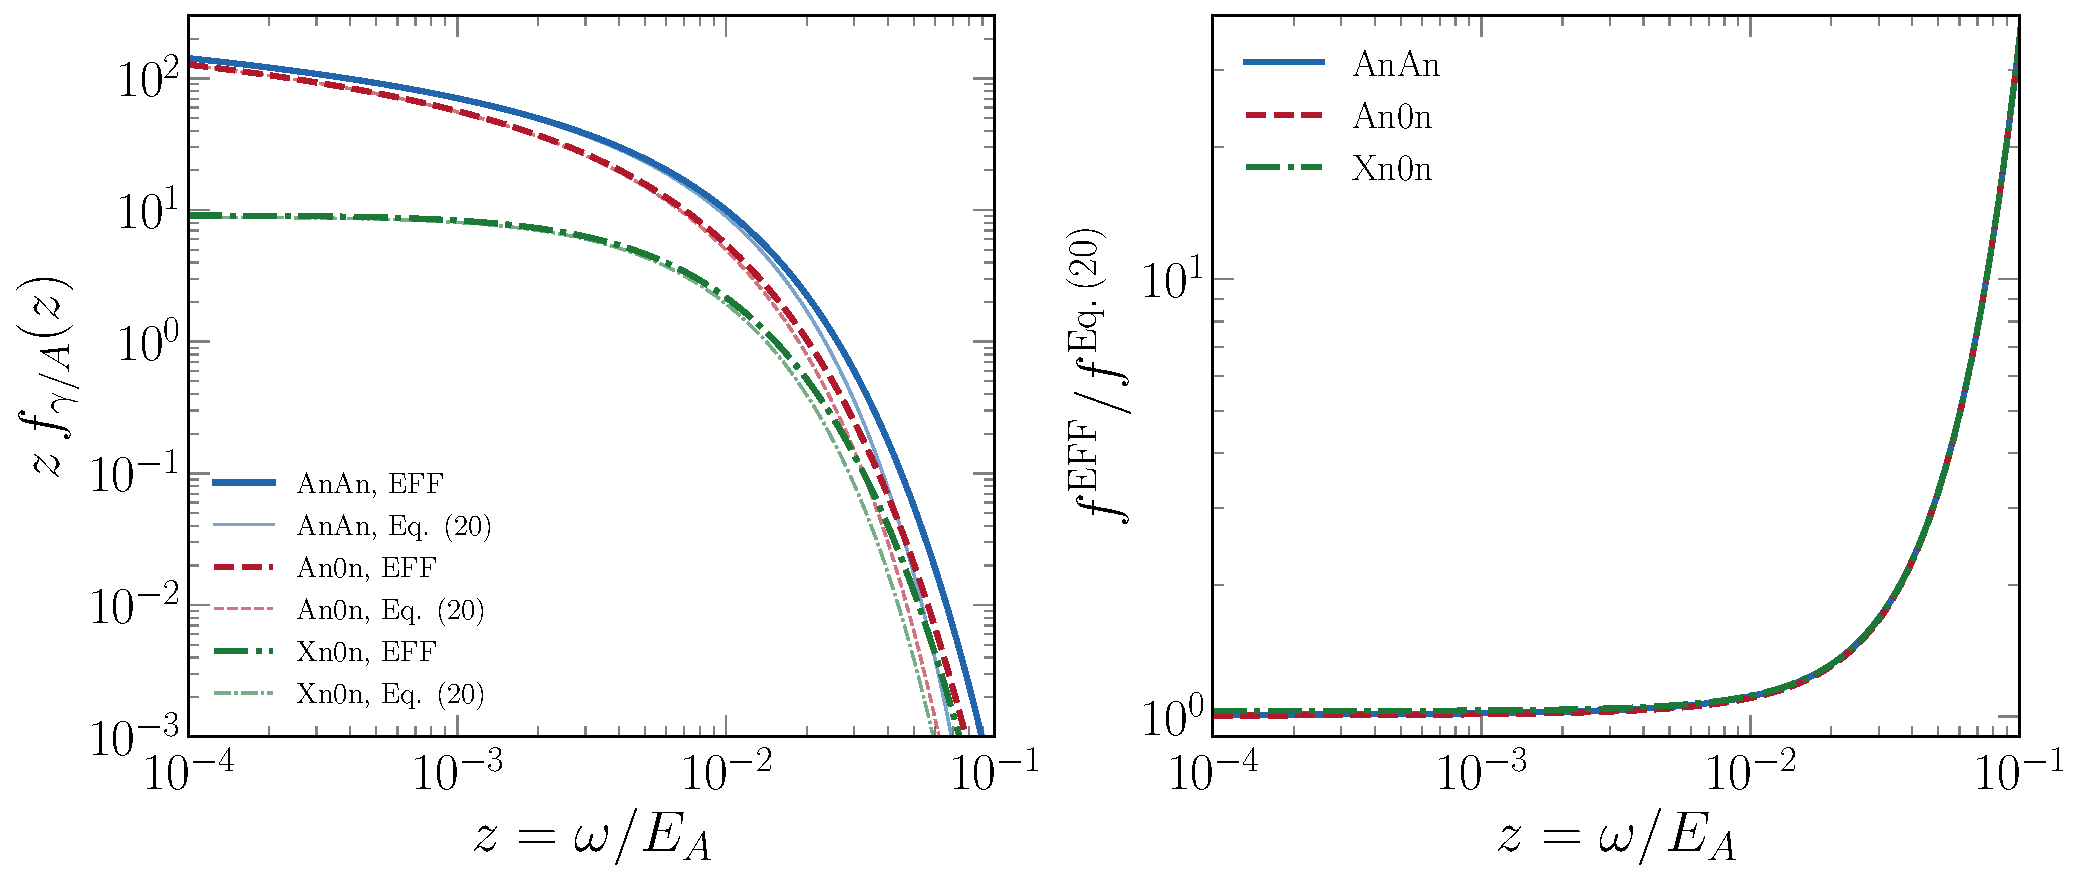
\includegraphics[width=\textwidth]{photon_flux_comparison_fig.pdf}
\caption{Left: $zf_{\gamma/A}(z)$ in Pb--Pb at 5.36 TeV with EFF (thick) and with GISS Eq.~(20)
(thin) for AnAn, An0n and Xn0n. Right: the ratio EFF/GISS, which is almost the same for the
three channels.}
\label{fig:flux}
\end{figure}

\paragraph{Where this matters for the D$^0$ results.} A charm quark with transverse mass
$m_T$ at rapidity $y$ needs $z\geq z_{\min}=m_Te^{y}/\sqrt{s_{NN}}$ (with $q^+\geq p^+$), and
because the flux falls steeply the cross section comes mostly from $z$ near $z_{\min}$. The
ratio at $z_{\min}$ is therefore a rough estimate of how much larger our cross sections are than
they would be with the GISS flux (an underestimate, since the ratio grows with $z$):

\begin{center}
\begin{tabular}{rrrccc}
\toprule
$p_\perp$ [GeV] & $y$ & $z_{\min}$ & AnAn & An0n & Xn0n \\
\midrule
 2 & 0 & $4.7\times10^{-4}$ & 1.01 & 1.01 & 1.03 \\
 5 & 0 & $9.7\times10^{-4}$ & 1.02 & 1.01 & 1.03 \\
10 & 0 & $1.9\times10^{-3}$ & 1.03 & 1.02 & 1.04 \\
 2 & 2 & $3.5\times10^{-3}$ & 1.04 & 1.03 & 1.05 \\
 5 & 2 & $7.2\times10^{-3}$ & 1.08 & 1.07 & 1.08 \\
10 & 2 & $1.4\times10^{-2}$ & 1.18 & 1.17 & 1.18 \\
10 & 3 & $3.8\times10^{-2}$ & 2.13 & 2.11 & 2.13 \\
\bottomrule
\end{tabular}
\end{center}

At low $p_\perp$ and central rapidity the difference is a few per cent; at high $p_\perp$ and
$y\gtrsim 2$ it is tens of per cent or more. The D$^0$ needs a charm quark with
$p_\perp > p_{D^0\perp}$, so $z_{\min}$ for a given $p_{D^0\perp}$ is somewhat larger than in the
table.

\section{Reproducing the GISS flux}

Run with \texttt{FLUX\_MODEL=WS} (Pb--Pb, with the default 92~mb $\Gamma_{AA}$ table). This is
GISS Eqs.~(15), (20) and (22): \texttt{photon\_flux()} evaluates
\texttt{flux\_density\_WS} at $r=b$ and multiplies it by $\Gamma_{AA}(b)$ and the channel factor,
and the code integrates over $b$. For p--Pb nothing needs to change.

\end{document}
